% !TEX program = xelatex
%
% Build:
%   xelatex slides.tex
%   xelatex slides.tex
%
% Requires: beamer, metropolis theme, ctex (Chinese), booktabs, tikz.
% Install hints:
%   sudo apt install texlive-xetex texlive-lang-chinese texlive-fonts-extra
% Or use Overleaf with compiler = XeLaTeX.

\documentclass[aspectratio=169,10pt]{beamer}

\usetheme[progressbar=frametitle,numbering=fraction]{metropolis}
\usepackage{ctex}
\usepackage{booktabs}
\usepackage{amsmath,amssymb}
\usepackage{xcolor}
\usepackage{tikz}
\usetikzlibrary{arrows.meta,positioning,fit,backgrounds}
\usepackage{graphicx}
\graphicspath{{figures/}}

\definecolor{mDarkTeal}{HTML}{23373B}
\definecolor{mLightBrown}{HTML}{EB811B}
\definecolor{mLightGreen}{HTML}{14B03D}
\setbeamercolor{alerted text}{fg=mLightBrown}

\title{Three-Layer View of Knowledge Corruption\\ in LLM Unlearning}
\subtitle{为什么要\emph{审计} forget set，而不是每次都 unlearn}
\date{}
\author{Bo \;|\; \texttt{unlearning/}}
\institute{Llama-3.1-8B-Instruct \;+\; GradAscent \;+\; WikiText-103 (HDBSCAN × 10)}

\begin{document}

\maketitle

% ────────────────────────────────────────────────────────────────────────────
\begin{frame}{一句话贡献}
    \begin{center}
        \Large
        Unlearning 的副作用沿语义距离\textbf{三层衰减，但不归零}。
    \end{center}

    \vspace{0.8em}
    \begin{center}
        \Large
        \textbf{L1 \;1.76×} \;→\; \textbf{L2 \;1.29×} \;→\; \textbf{L3 \;1.16×}
    \end{center}

    \vspace{0.8em}
    \begin{center}
        \normalsize
        且 \alert{61.6\,\%} 的「无关」样本 PPL 也被抬高。
    \end{center}

    \vfill
    \footnotesize\itshape\centering
    Llama-3.1-8B-Instruct · GradAscent · $n=10$ forget sets.
\end{frame}

% ────────────────────────────────────────────────────────────────────────────
\section{动机与定义}

\begin{frame}{动机：一句话}
    \vfill
    \begin{center}
        \Large
        换个 forget set，副作用能差 \textbf{1.7×}。
    \end{center}

    \vspace{0.6em}
    \begin{center}
        \normalsize
        可每跑一个 unlearn 要数 GPU-hour。
    \end{center}

    \vspace{1.0em}
    \begin{center}
        \Large
        \alert{能不能不 fine-tune，就预测副作用？}
    \end{center}
    \vfill
\end{frame}

\begin{frame}{三层是什么：一张同心圆图}
    \centering
    \begin{tikzpicture}[font=\small]
        \fill[mDarkTeal!10]    (0,0) circle (3.2);
        \fill[mLightBrown!30]  (0,0) circle (2.0);
        \fill[mLightBrown!60]  (0,0) circle (1.0);
        \draw[thick] (0,0) circle (1.0);
        \draw[thick] (0,0) circle (2.0);
        \draw[thick, dashed] (0,0) circle (3.2);

        \node at (0, 0.0)    {\textbf{\Large L1}};
        \node at (0, 1.5)    {\textbf{\Large L2}};
        \node at (0, 2.6)    {\textbf{\Large L3}};

        \draw[-Latex, thick] (3.4, 0.0) -- node[right, align=left]
            {\textbf{L1} 想遗忘的\\ \footnotesize 被 unlearn 那批} (1.2, 0.0);
        \draw[-Latex, thick] (3.7, 1.5) -- node[right, align=left]
            {\textbf{L2} 连带忘的\\ \footnotesize 同 cluster · 没训过} (2.1, 1.5);
        \draw[-Latex, thick] (4.0, 2.7) -- node[right, align=left]
            {\textbf{L3} 不该忘却被波及\\ \footnotesize 别的 cluster} (3.1, 2.7);

        \node[left, font=\footnotesize] at (-3.3, 0) {离 forget set 越远};
        \draw[-Latex, thick, mDarkTeal] (-3.3, 0.3) -- (-3.3, 2.5);
        \node[left, font=\footnotesize] at (-3.3, 2.8) {副作用应越小};
    \end{tikzpicture}
\end{frame}

\begin{frame}{怎么量化：一个比值}
    \vfill
    \begin{center}
        \Large
        $r \;=\; \dfrac{\text{PPL}_\text{unlearned}}{\text{PPL}_\text{base}}$
    \end{center}

    \vspace{0.8em}
    \begin{center}
        \large
        $r = 1.8$ $\Rightarrow$ 这条样本的 PPL 被抬高到 \textbf{1.8 倍}。
    \end{center}

    \vspace{0.8em}
    \begin{center}
        \normalsize
        每一层取几何均值 $\Rightarrow$ 得到 L1 / L2 / L3 的一个数。
    \end{center}
    \vfill
\end{frame}

% ────────────────────────────────────────────────────────────────────────────
\begin{frame}{数据怎么来：四步}
    \centering
    \begin{tikzpicture}[
        node distance=3.5mm,
        box/.style={draw, rounded corners=2pt, align=center,
                    minimum height=10mm, text width=30mm, font=\small},
        arr/.style={-Latex, thick, mDarkTeal},
    ]
        \node[box, fill=mDarkTeal!12] (c) {WikiText-103\\聚成 \textbf{10 簇}};
        \node[box, fill=mDarkTeal!12, right=6mm of c] (t) {每簇 1 个\\ forget set};
        \node[box, fill=mLightGreen!20, right=6mm of t] (u) {\textbf{10 次}\\ unlearn};
        \node[box, fill=mLightBrown!25, right=6mm of u] (m) {\textbf{10×10}\\ cross-ppl};

        \draw[arr] (c) -- (t);
        \draw[arr] (t) -- (u);
        \draw[arr] (u) -- (m);
    \end{tikzpicture}

    \vspace{1.4em}
    \centering
    \large
    10×10 矩阵的\textbf{对角线} = L1 + L2\quad\textbf{非对角线} = L3
\end{frame}

% ────────────────────────────────────────────────────────────────────────────
\section{第一幕 · 数据证实三层 View}

\begin{frame}{这一幕要说服你三件事}
    \vspace{0.8em}
    \begin{description}
        \setlength\itemsep{0.8em}
        \item[\alert{C1}] 三层\textbf{严格递减}（L1 > L2 > L3），不是乱分箱。
        \item[\alert{C2}] L3 \textbf{不是 0}：无关样本也真被波及。
        \item[\alert{C3}] profile \textbf{随 forget set 变化}，所以\emph{值得审计}。
    \end{description}
\end{frame}

\begin{frame}{C1 + C2：headline 数字}
    \vspace{0.3em}
    \centering
    \begin{tabular}{@{}lccc@{}}
        \toprule
        & L1 forget & L2 locality & L3 spillover \\
        \midrule
        geo-mean $r$           & \textbf{1.76×} & \textbf{1.29×} & \textbf{1.16×} \\
        被抬高（$>1.1×$）占比    & 95.6\,\%       & 82.8\,\%       & \alert{61.6\,\%} \\
        \bottomrule
    \end{tabular}

    \vspace{1.2em}
    \begin{center}
        \large
        \textbf{C1 成立}：1.76 $>$ 1.29 $>$ 1.16\\[0.4em]
        \textbf{C2 成立}：L3 仍有 \alert{61.6\,\%} 样本被抬高
    \end{center}
\end{frame}

\begin{frame}{C1 + C2：一图}
    \centering
    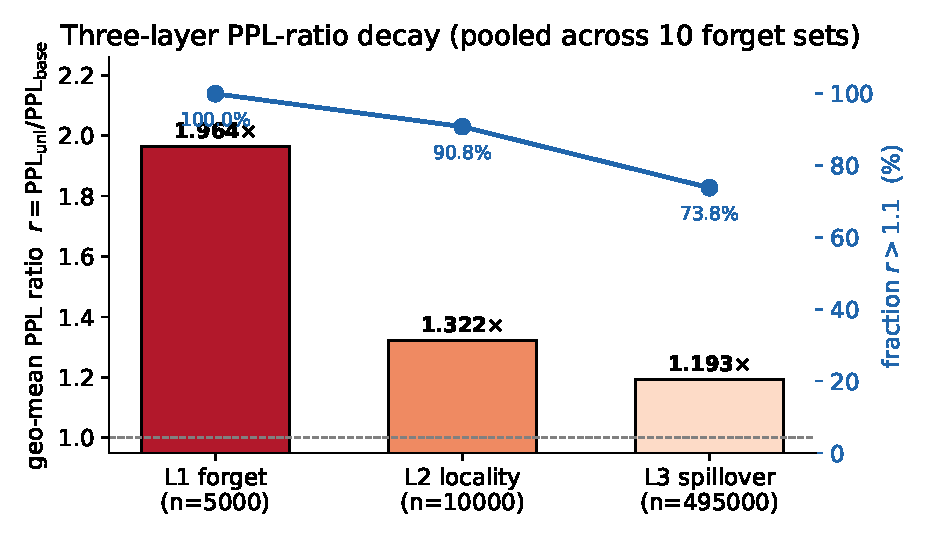
\includegraphics[width=0.82\textwidth]{fig_three_layer_decay.pdf}

    \vspace{0.3em}
    \footnotesize
    左轴：L1 $>$ L2 $>$ L3\quad|\quad右轴：L3 仍有 \alert{61.6\,\%} 被抬高。
\end{frame}

\begin{frame}{C3：换个 forget set，副作用差多少？}
    \centering
    \small
    \begin{tabular}{@{}lccc@{}}
        \toprule
        & L1 & L2 & L3 \\
        \midrule
        最温和（\texttt{star}）    & 1.42 & 1.12 & 1.07 \\
        \alert{最严重（\texttt{storm}）} & \alert{\textbf{2.44}} & \alert{\textbf{1.78}} & \alert{\textbf{1.25}} \\
        \midrule
        极差比                    & \textbf{1.72×} & 1.60× & 1.17× \\
        \bottomrule
    \end{tabular}

    \vspace{1.2em}
    \begin{center}
        \Large
        同一算法，换 forget set，L1 副作用差 \alert{\textbf{1.7×}}。
    \end{center}

    \vspace{0.4em}
    \begin{center}
        \normalsize
        $\Rightarrow$ profile 是 forget set 的函数，值得\emph{审计}。
    \end{center}
\end{frame}

\begin{frame}{C3：一图}
    \centering
    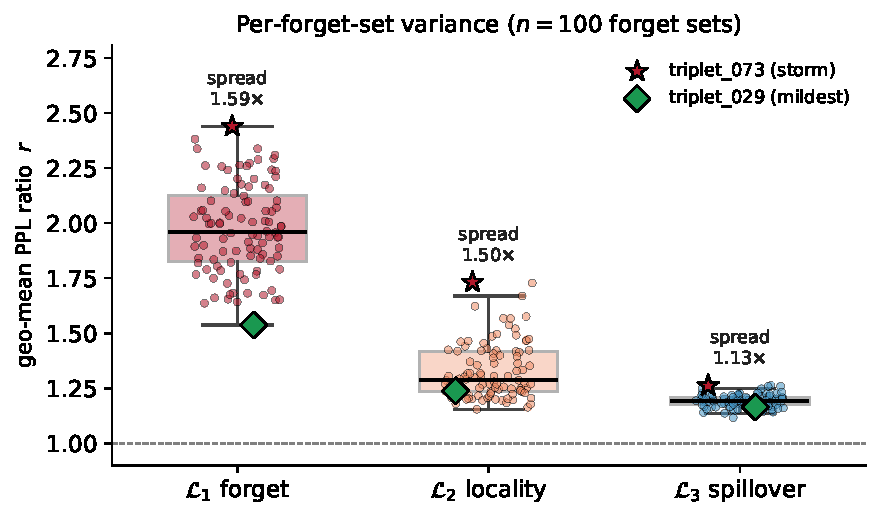
\includegraphics[width=0.88\textwidth]{fig_per_forget_profile.pdf}

    \vspace{0.3em}
    \footnotesize
    按 L1 升序；\alert{storm} 三层同时最严重 $\Rightarrow$ 稳健坏 forget set。
\end{frame}

% ────────────────────────────────────────────────────────────────────────────
\section{第二幕 · 与其每次 unlearn，不如审计}

\begin{frame}{审计问题：输入是什么、输出是什么}
    \vspace{0.4em}
    \begin{center}
        \begin{tikzpicture}[font=\small, node distance=10mm]
            \node[draw, rounded corners, fill=mDarkTeal!12, minimum width=32mm, minimum height=12mm, align=center] (in)
                {\textbf{输入}\\ forget set 的\\ 12 维几何特征};
            \node[draw, rounded corners, fill=mLightGreen!25, right=16mm of in, minimum width=28mm, minimum height=12mm, align=center] (box) {\textbf{审计器}\\ Ridge};
            \node[draw, rounded corners, fill=mLightBrown!25, right=16mm of box, minimum width=32mm, minimum height=12mm, align=center] (out)
                {\textbf{输出}\\ L1 / L2 / L3\\ 三个风险分数};
            \draw[-Latex, thick] (in) -- (box);
            \draw[-Latex, thick] (box) -- (out);
        \end{tikzpicture}
    \end{center}

    \vspace{0.8em}
    \begin{center}
        \large
        \alert{不看 evaluation · 不跑 unlearn}
    \end{center}

    \vspace{0.6em}
    \footnotesize\centering
    12 维 = 方差 / 两两相似度 / centroid / 集中度（effective rank, isotropy）。\\
    10 forget set 上 Leave-One-Out。
\end{frame}

\begin{frame}{审计结果}
    \centering
    \begin{tabular}{@{}lccc@{}}
        \toprule
        & L1 forget & L2 locality & L3 spillover \\
        \midrule
        $R^2$           & \textbf{+0.44} & \textbf{+0.41} & +0.19 \\
        排序 Spearman $\rho$ & +0.62 & +0.62 & +0.61 \\
        Top-1 命中       & \alert{\checkmark \, storm} & $\times$ & $\times$ \\
        \bottomrule
    \end{tabular}

    \vspace{1.2em}
    \begin{center}
        \Large
        三层排序相关 $\rho \approx \textbf{0.62}$
    \end{center}
    \vspace{0.3em}
    \begin{center}
        \normalsize
        L1 最严重的 forget set (\texttt{storm}) 被正确预测到。
    \end{center}

    \vspace{0.4em}
    \footnotesize\centering\itshape
    $n=10$，单观察点；$n\uparrow$、换 unlearner 的稳健性待验证。
\end{frame}

\begin{frame}{审计散点：预测 vs 真实}
    \centering
    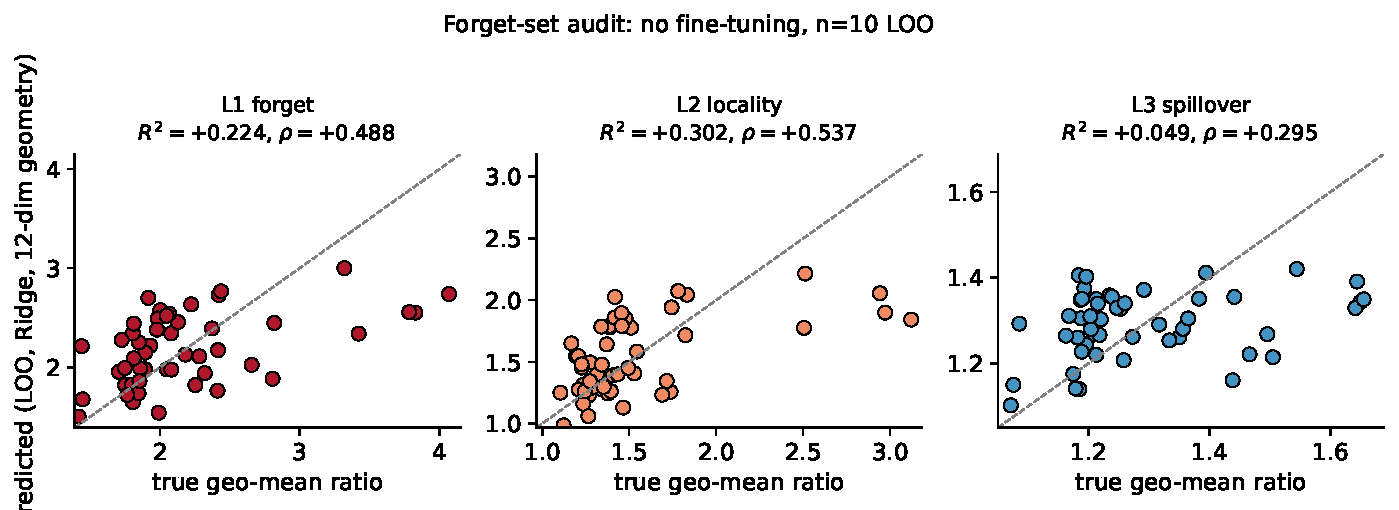
\includegraphics[width=0.96\textwidth]{fig_audit_scatter.pdf}

    \vspace{0.2em}
    \footnotesize
    虚线 $y=x$；三层 $\rho \approx 0.62$；L3 幅度小、排序仍可用。
\end{frame}

\begin{frame}{几何 vs 文本表面}
    \centering
    \begin{tabular}{@{}lcc@{}}
        \toprule
        特征 & 维度 & $R^2$ \\
        \midrule
        文本表面统计        & 261          & +0.14 \\
        \textbf{纯几何}     & \textbf{16}  & \textbf{+0.36} \\
        \bottomrule
    \end{tabular}

    \vspace{1.2em}
    \begin{center}
        \Large
        特征少 \alert{16×}，$R^2$ 高 \alert{2.5×}
    \end{center}

    \vspace{0.4em}
    \begin{center}
        \normalsize
        corruption 更像\emph{几何}现象，而非文本难度现象。
    \end{center}
\end{frame}

\begin{frame}{诚实负结果：球覆盖不 work}
    \vspace{0.5em}
    \begin{center}
        \large
        试过：用 forget set 的半径圈 retain，看落入比例。
    \end{center}

    \vspace{0.8em}
    \begin{center}
        \large
        结果：与真实 L3 的相关 $\rho = \alert{-0.42}$（\textbf{方向反了}）
    \end{center}

    \vspace{0.8em}
    \begin{center}
        \normalsize
        原因：簇之间互相重叠，球太大 $\Rightarrow$ 几乎全覆盖。\\[0.3em]
        改进：带符号投影 / mutual-reachability 距离。
    \end{center}
\end{frame}

% ────────────────────────────────────────────────────────────────────────────
\section{讨论}

\begin{frame}{Related Work}
    \begin{center}
        \large
        相邻工作与我们的差别
    \end{center}

    \vspace{0.6em}
    \small
    \begin{tabular}{@{}p{0.34\textwidth}p{0.58\textwidth}@{}}
        \toprule
        相邻方向 & 我们的差别 \\
        \midrule
        Data-first 鲁棒性\newline (Dang+ ACL'24) & 训练集特征 $\to$ 对抗 ASR \newline\; $\Rightarrow$ 迁到 \emph{unlearning corruption} \\
        LLM unlearning 算法 & 我们固定 unlearner，分析\emph{数据依赖}的副作用 \\
        Influence / editing\newline locality & model-centric $\to$ \emph{data-centric} 三层风险 \\
        \bottomrule
    \end{tabular}
\end{frame}

\begin{frame}{Limitations}
    \vspace{0.3em}
    \begin{center}
        \large
        四个「单」
    \end{center}

    \vspace{0.6em}
    \begin{itemize}
        \setlength\itemsep{0.6em}
        \item 单 base model（Llama-3.1-8B-Instruct）
        \item 单 unlearner（GradAscent）
        \item 单 $n = 10$ forget sets（CI 较宽）
        \item 单指标 PPL（$\neq$ QA 准确率）
    \end{itemize}
\end{frame}

\begin{frame}{Future Work}
    \vspace{0.3em}
    \begin{center}
        \large
        对应四个「单」的解法
    \end{center}

    \vspace{0.6em}
    \begin{enumerate}
        \setlength\itemsep{0.5em}
        \item $n: 10 \to 100$（100 triplet 已生成）
        \item 加 NPO / GradDiff 验证审计器稳健
        \item PPL $\to$ QA accuracy（\texttt{2.extract-qa/} 已就位）
        \item \emph{audit-driven} forget 选择：挑预测 L3 最低的 $\mathcal{D}_f$
    \end{enumerate}
\end{frame}

\begin{frame}{论文定位}
    \begin{center}
        \large
        \emph{A Three-Layer View of Knowledge Corruption\\ in LLM Unlearning.}
    \end{center}

    \vspace{0.8em}
    \textbf{三个卖点}
    \begin{enumerate}
        \item 三层 view + L3 61.6\,\% $\Rightarrow$ spillover \emph{不可忽略}
        \item benchmarking $\to$ \textbf{forget-set audit} 视角转换
        \item 仅几何就能排序预测（$\rho \approx 0.62$）
    \end{enumerate}

    \vspace{0.6em}
    \begin{center}
        \small
        \textbf{升档}：$n$=10 $\to$ 100 + 第二个 unlearner $\Rightarrow$ NeurIPS / ICML
    \end{center}
\end{frame}

% ────────────────────────────────────────────────────────────────────────────
\begin{frame}[standout]
    三层衰减，但不归零。\\[0.5em]
    \normalsize
    \textbf{1.76× → 1.29× → 1.16×}\\[0.3em]
    审计 $\rho \approx 0.62$，无需 unlearn。
\end{frame}

\appendix

\begin{frame}[fragile]{附录 — 复现主结果}
    \footnotesize
\begin{verbatim}
# 0. Unlearn 与 cross-ppl（已完成可跳过）
#    ⇒ 2.extract-ppl/wikitext_cross_metrics_detail.json

# 1. 第一幕：三层 ground truth
cd 2.extract-ppl
python analyze_corruption.py          # ⇒ corruption_summary.json

# 2. 第二幕 A：per-sample 几何预测器
cd ../4.regression-predictor
python 3.corruption_from_geometry.py  # ⇒ geometry/geometry_results.json

# 3. 第二幕 B：forget-set 审计（LOO, Part 1+2+3+3b）
python 4.audit_experiments.py         # ⇒ audit/audit_summary.json
\end{verbatim}
\end{frame}

\begin{frame}{附录 — 关键 artefact}
    \footnotesize
    \begin{tabular}{@{}ll@{}}
        \toprule
        Artefact & 路径 \\
        \midrule
        Cross-eval ppl 明细 & \texttt{2.extract-ppl/wikitext\_cross\_metrics\_detail.json} \\
        三层 corruption 汇总 & \texttt{2.extract-ppl/corruption\_summary.json} \\
        几何 per-sample 预测 & \texttt{4.regression-predictor/geometry/geometry\_results.json} \\
        审计器 LOO 预测 & \texttt{4.regression-predictor/audit/audit\_summary.json} \\
        每 forget set L1/L2/L3 & \texttt{audit/part1\_corruption\_profile.csv} \\
        审计特征表 & \texttt{audit/part2\_forget\_features.csv} \\
        \bottomrule
    \end{tabular}
\end{frame}

\end{document}
